% Template for ISBI paper; to be used with:
%          spconf.sty  - ICASSP/ICIP LaTeX style file, and
%          IEEEbib.bst - IEEE bibliography style file.
% --------------------------------------------------------------------------
\documentclass{article}
\usepackage{spconf,amsmath,graphicx}
\usepackage{url}
% It's fine to compress itemized lists if you used them in the
% manuscript
\usepackage{enumitem}
\setlist{nosep, leftmargin=14pt}

\usepackage{mwe} % to get dummy images

% Example definitions.
% --------------------
\def\x{{\mathbf x}}
\def\L{{\cal L}}

% Title.
% ------
\title{Simultaneous Segmentation of Multiple Structures in Fundal Images using Deep Neural Networks}
%
% Single address.
% ---------------
%\name{Sunil Kumar Vengalil}
%\address{International Institute of Information Technology}
%
% For example:
% ------------
%\address{School\\
%	Department\\
%	Address}
%
% Two addresses (uncomment and modify for two-address case).
% ----------------------------------------------------------
%\twoauthors
%  {A. Author-one, B. Author-two\sthanks{Some author footnote.}}
%	{School A-B\\
%	Department A-B\\
%	Address A-B}
%  {C. Author-three, D. Author-four\sthanks{The fourth author performed the work
%	while at ...}}
%	{School C-D\\
%	Department C-D\\
%	Address C-D}
%
% More than two addresses
% -----------------------
% \name{Sunil Kumar Vengalil^{\star \dagger}$ \qquad Bharath K^{\star}$ \qquad Neelam Sinha^{\dagger}$}
%
% \address{$^{\star}$ International Institute of Information Technology \\
%     $^{\dagger}$}Affiliation Number Two
%
\begin{document}
%\ninept
%
\maketitle
%
\begin{abstract}
Fundal imaging is the most commonly used non-invasive technique for early detection of many retinal diseases like diabetic retinopathy.
An initial step in automatic processing of fundal images for detecting diseases is to identify the various landmark regions like optic disc, blood vessels and fovea.
In addition to these, various abnormalities like exudates that help in pathological analysis are also visible in fundal images.
In this work, we propose a multi-tasking deep learning architecture for segmenting optic disc, blood vessels, fovea and exudates simultaneously.
Our experimental results on publicly available datasets show that simultaneous segmentation of all these structures results in significant improvement in the performance.
For segmentation performance on blood vessels, optic disc, fovea and exudates, we got a Dice score of 78.5\%, 94\%, 66\% and 60\% respectively.
Proposed simultaneous segmentation approach resulted in a peak  improvement of 10\%  on the exudates segmentation task compared to the individual segmentation using the same network architecture.
To the best of our knowledge, we  are the first one to evaluate the effectiveness of  multi-task learning for segmenting multiple structures in fundal images.
We obtained a state of the art Dice score of 78\% for blood vessel segmentation on 20 DRIVE test images which is 2\% higher than one of the recently reported studies.
\end{abstract}
%
\begin{keywords}
Fundal Image Segmentation, Multi-task learning, Deep Learning
\end{keywords}
%

\section{Introduction}
Fundal imaging, capturing images of retina using specialized cameras, is the most widely used non-invasive technique for screening of retinal diseases.
These images are used to identify common eye diseases like diabetic retinopathy, which is the most common cause for blindness, and many other cardiovascular diseases.
Blood vessels, optic disc and fovea are the major structures visible in a fundal image.
However, manual identification and demarcation of fine structures like blood vessels take a lot of time and effort.
Hence automatic detection of major landmarks in fundal image has become an active research area.

Figure \ref{sample_funal_image} shows a fundal image with various structures like blood vessels, optic disc and fovea marked.
The optic disc is the point of exit of the optic nerves that carry information from the eye to the brain.
It is also the point where all the blood vessels enter the eye.
Since there are no photo sensors (rods and cones) present in the optic disc, it corresponds to a blind spot in the retina.
Fovea is a small region with a lot of cone cells packed together and hence this region is responsible for sharp vision.
Blood vessels that carry blood to the eye are spread across the entire region of the retina and vary in thickness and density.

Since the break-through success of deep learning in solving tasks in domains like computer vision for classification \cite{krizhevsky2012imagenet} \cite{simonyan2014very} and segmentation \cite{chen2017deeplab}, many deep learning architectures have been tried for segmenting important structures, such as optic disc and blood vessels, in fundal images \cite {vengalil2016customizing} \cite{zhuang2018laddernet} \cite{jiang2018retinal} \cite{park2020m}.
One of the challenges of using deep learning architecture for medical images is the lack of annotated training data.
Many approaches, like taking multiple training patches from  a single image \cite{vengalil2016customizing} and transfer learning, where a model trained on a dataset such as the Imagenet \cite{deng2009imagenet} is fine tuned for the task at hand, are proposed and found to be successful.

In this work, we propose a multi-tasking deep learning architecture for simultaneous detection of blood vessels, optic disc, fovea and exudates.
Our results show that a single network that predicts multiple structures  performs much better compared to detecting  each structure independently using different networks as the single network can make use of the correlation between the two tasks.
This correlation is evident from Figure \ref{sample_funal_image}, where one can see that near and inside the optic disc blood vessels are thicker and denser.
So the knowledge of the optic disc can help the prediction task for blood vessels and vice versa.
We perform experiments and report results on three popular datasets DRIVE \cite{drive}, HRF \cite{budai2013robust} and IDRID \cite{h25w98-18}.

The contribution of our work are:
\begin{enumerate}
  \item Propose a multi-tasking model for simultaneous segmentation of blood vessels, optic discs, fovea and exudates.
  \item Propose a method for data augmentation of fundal images which enables the training and prediction on whole images, rather than using image patches.
  Using the entire image provides more contextual information that can help the segmentation task.
  \item We report a state of the art accuracy of 78\% on DRIVE test images which is 2\% higher than the results reported by Adapa et al.\cite{adapa2020supervised}.
\end{enumerate}

\begin{figure}[!ht]
  \centering
  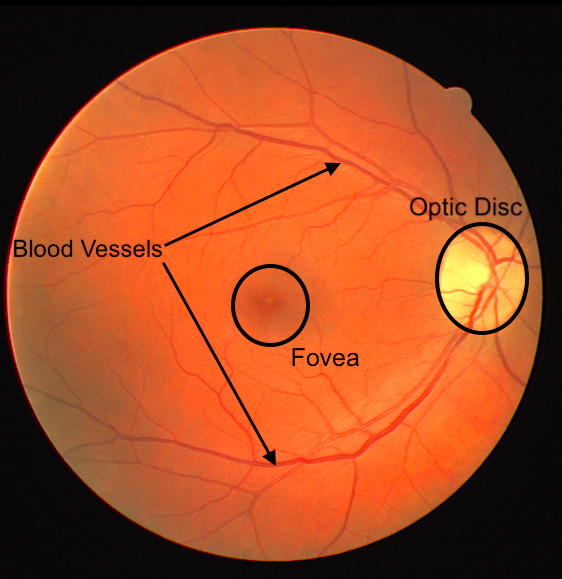
\includegraphics[width=0.5\linewidth]{images/eye_1.png}
  \caption{Sample fundal image showing important structures}
  \label{sample_funal_image}
\end{figure}

\section{Related Work}
Existing  techniques for fundal image segmentation mainly fall under two categories 1) using traditional image processing techniques and 2) using deep learning techniques.
Examples of image processing based techniques include filter based \cite{zhang2010retinal} \cite{yavuz2011retinal} \cite{aslan2018segmentation} and morphological operations based \cite{hassan2015retinal}\cite{singh2014new}.
Image processing based techniques have the advantage that they don’t need the ground truth images, but their performance is far behind the deep learning based approaches.
Further, these algorithms are based on many tunable thresholds that vary from dataset to dataset and they work based on some assumptions like gaussian distribution.

Several deep learning architectures that were successful in segmentation tasks \cite{chen2017deeplab} in natural images were tried for segmenting blood vessels in retinal images and the results were significantly better than using conventional image processing techniques.
In \cite{vengalil2016customizing} a state-of-the-art segmentation model deeplab \cite{chen2017deeplab}, which is pre-trained on natural images  for semantic segmentation,  was used to segment blood vessels at pixel level.
Jiang et.al. proposes \cite {jiang2018retinal} a  pre-trained fully convolutional network for segmenting blood vessels and report accuracy of cross-dataset test on four different datasets.
In M-GAN \cite{park2020m}, introduced by Kyeong et.al., a multi-kernel pooling block added between stacked convolutional layers supports scale-invariance which is a highly desirable feature for blood vessel segmentation.

One of the main challenges in using deep neural networks for segmentation tasks is that the reduction in resolution of featuremap as one goes deeper will result in loss of finer details like edges, which are crucial for segmentation tasks.
In order to circumvent this, the U-Net \cite{ronneberger2015u} model was introduced specifically for medical image segmentation which has multiple skip connections.
In their recent work, Joshua et.al. \cite{joshua2020blood} used a modified version of U-NET for segmenting blood vessels in retinal images and reported state of the art accuracies.
In Laddernet, introduced by Zhuang et.al. in 2018 \cite{zhuang2018laddernet},  is a sequence of multiple U-Nets cascaded together.

\section{Proposed Method}
A modified version of the UNET architecture \cite{ronneberger2015u}, shown in Fig \ref{unet_combined}, was used for segmenting various structures.
The encoder and decoder consists of 4 stages each.
Each stage of the encoder comprises two convolution layers, each followed by batch normalization and ReLU activation function.
A max-pooling layer with a stride of 2 was added at the end of each stage of the encoder which down samples the image by a factor of two.
Each decoder layer up-samples the image by a factor of 2 using  a deconvolution layer followed by a convolution layer.

For experiments on individual prediction the network had one output channel corresponding to the segmentation map.
The network outputs a binary image, of the same resolution as the input,  which indicates pixel by pixel segmentation.
For multi-tasking models an additional channel, for predicting the optic disc in combination with another structure,  was added at the output layer.
We chose to combine optic disc with other structures as optic disc annotation was available for all the datasets.

\begin{figure}[!ht]
  \centering
  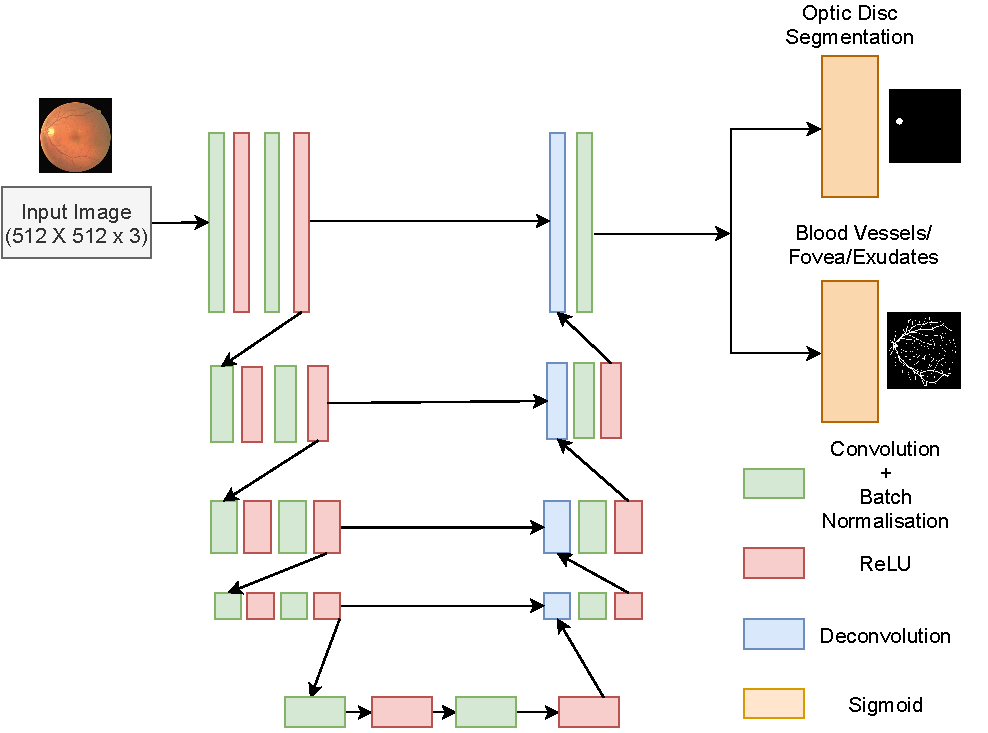
\includegraphics[width=0.9\linewidth]{images/UnetArch.pdf}
  \caption{Architecture of the proposed multi-tasking U-Net model}
  \label{unet_combined}
\end{figure}

\vspace{-0.2in}
\subsection{Dataset}
We used the DRIVE \cite{drive} and HRF \cite{budai2013robust}  datasets for blood vessel segmentation and optic disc segmentation. The DRIVE dataset contains 20 training images and 20 testing images of resolution $565 \times 584$ pixels. The dataset also provides ground truth images for blood vessel segmentation annotated by a human expert. As the DRIVE dataset does not have optic disc annotations, we annotated the optic disc in each image ourselves. HRF dataset has 15 high resolution fundal images along with ground truth annotation for blood vessel segmentation.

IDRID \cite{h25w98-18} localization dataset, which contains  413 training images and 103 test images along with fovea ground truth, was used for fovea localization.
For exudates segmentation, we used IDRID \cite{h25w98-18} segmentation dataset which contains a total of 81 images.

We used full images, as opposed to image patches, for training the network  as a full image will have more context and hence can be more effective for predicting structures like optic disc and fovea.
Data-augmentation - horizontal and vertical flipping, grid and elastic distortion provided by the library Albumentations \cite{buslaev2020albumentations},
was used  to increase the number of training samples by a factor of 4.

\subsection{Loss function and training}\label{sec:loss_and_training}
A sigmoid activation function is used at the output layer. The model is trained with dice loss and adam optimizer.
For predicting the structures separately, four separate networks with the same architecture were trained independently one for each of the structures: blood vessel, optic disc, fovea and exudates.

In the multi-tasking model, we trained three separate networks each with two output channels for predicting the following three combinations:
\begin{enumerate}
  \item Blood vessel and  optic disc
  \item Fovea and optic disc
  \item Exudates and optic disc
  \end{enumerate}

The network was trained for 60 epochs in all the cases.

\begin{figure}[!ht]
  \begin{minipage}[b]{0.7\linewidth}
  \centering
  \centerline{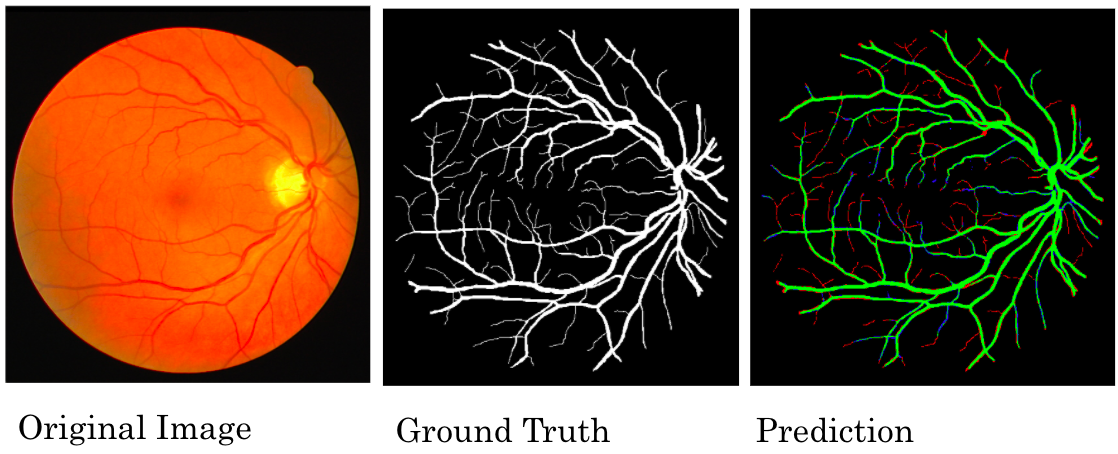
\includegraphics[width=6cm]{images/bv_prediction.png}}
  \centerline{(a) Blood Vessels}\medskip
  \end{minipage}

  \begin{minipage}[b]{0.7\linewidth}
  \centering
  \centerline{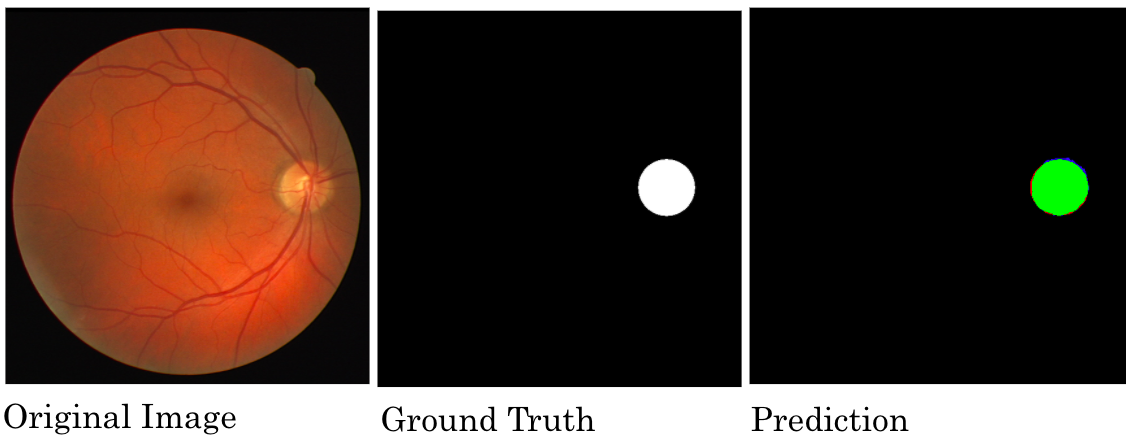
\includegraphics[width=6cm]{images/od.png}}
  \centerline{(b) Optic Disc}\medskip
  \end{minipage}

  \begin{minipage}[b]{0.7\linewidth}
  \centering
  \centerline{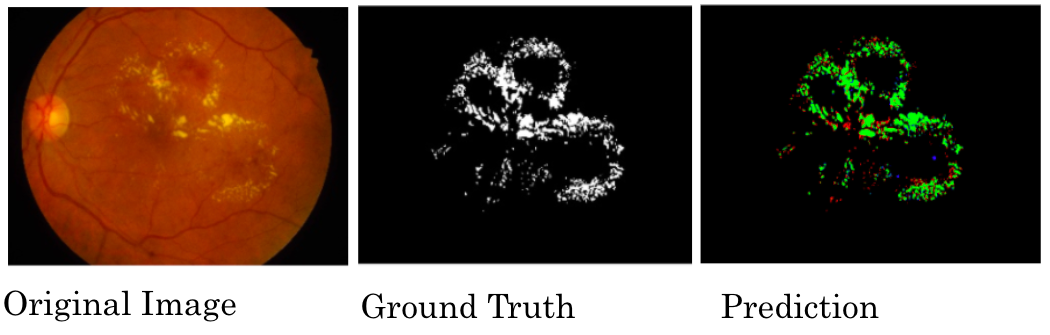
\includegraphics[width=6cm]{images/ex.png}}
  \centerline{(c) Exudates}\medskip
  \end{minipage}

  \begin{minipage}[b]{0.7\linewidth}
  \centering
  \centerline{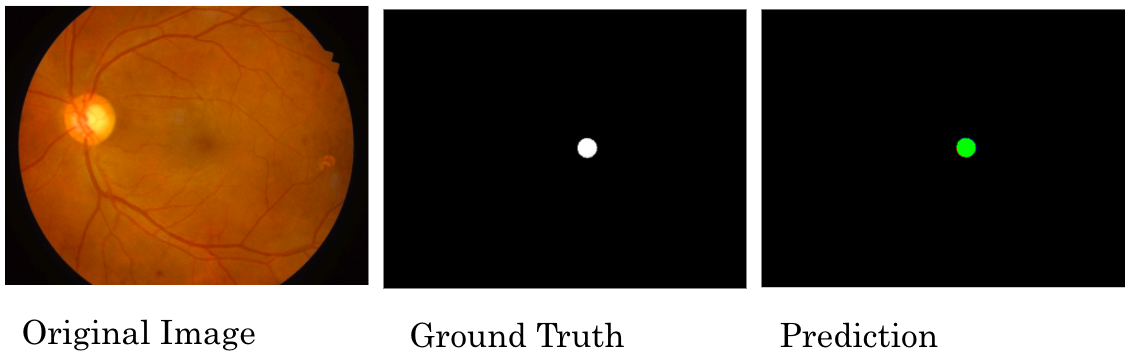
\includegraphics[width=6cm]{images/fovea.png}}
  \centerline{(d) Fovea}\medskip
  \end{minipage}

  \caption{Sample segmentation results. The green pixels in the predicted image correspond to true positives, blue pixels correspond to false positives and  red pixels correspond to false negatives.}
  \label{fig:segmentation_results}

\end{figure}

\section{Results and Discussion}\label{sec:results}
\vspace{-0.2in}
\begin{table}[htbp]
\caption{Comparison of results with and without multi-tasking}
\begin{center}
\begin{tabular}{|c|c|c|c|c|c|}
\hline
&&\multicolumn{2}{|c|}{\textbf{Individual}}& \multicolumn{2}{|c|}{\textbf{Multi-tasking}} \\
\cline{3-6}
 &\textbf{\textit{Dataset}}& \textbf{\textit{Dice}}& \textbf{\textit{IoU}}& \textbf{\textit{Dice}}& \textbf{\textit{IoU}}  \\
\hline
Blood Vessel&DRIVE &0.72&0.60 &0.78&0.63  \\
\cline{2-6}
&HRF&0.78&0.62&0.79&0.63 \\
\hline
Optic Disc& DRIVE&0.71&0.62 &0.76&0.63  \\
\cline{2-6}
&IDRID&0.88&0.81&0.94&0.9 \\
\hline
Fovea&IDRID&0.70&0.61 &0.66 &0.57  \\
\hline
Exudates&IDRID&0.50&0.34 &0.6&0.45  \\
\hline
\end{tabular}
\label{tab:results}
\end{center}
\end{table}

Table \ref{tab:results} summarises performance metrics on all the segmentation tasks on various datasets.
As evident from the table,  Dice score for exudates segmentation resulted in an improvement  of 10\% by the proposed multi-tasking approach.
A similar trend is observed in blood vessel and optic disc segmentation also with an improved Dice score of 6\%.
The increase in Dice score is due to less number of false positives in the prediction( resulting in larger precision).


The improved performance with multi-tasking is a consequence of direct correlation between the two predicted structures.
When trained together, the network is able to learn new hidden layer features that can contribute to the prediction of both structures.
When trained individually, the optic disc can easily be confused as exudates.
In simultaneous segmentation, the network learns to discriminate optic disc and exudates which improves the segmentation results for both.

Figure \ref{fig:segmentation_results} shows sample segmentation output for  blood vessels, optic disc, fovea and exudates with multi-tasking loss function.

\section{Conclusion}
In this work, we illustrate the effectiveness of multi-tasking deep learning models for segmenting blood vessels, optic disc, fovea and exudates in fundal images.
We build a multi-tasking model, and corresponding loss function,  based on the famous U-Net architecture for simultaneous  segmentation of multiple structures.
Using the proposed approach we report a Dice score of 78.5\%, 94\%, 66\% and 60\% on segmentation of blood vessels, optic disc, fovea and exudates respectively.
The proposed approach resulted in  a peak increase of 10\% in Dice score for exudates segmentation compared to the individual segmentation result with the same architecture.
Using the proposed approach we were able to get a state of the art accuracy of 78\% on DRIVE test images which is 2\% greater than one of the recently reported results.

\section{Compliance with ethical standards}
\label{sec:ethics}
No ethical approval was required for this study as we used only publicly available datasets.
%% References should be produced using the bibtex program from suitable
%% BiBTeX files (here: strings, refs, manuals). The IEEEbib.bst bibliography
%% style file from IEEE produces unsorted bibliography list.
%% -------------------------------------------------------------------------
\bibliographystyle{IEEEbib}
\bibliography{strings,refs}

\end{document}
